\documentclass{standalone}
\usepackage{tikz}
\usepackage{pgfplots}
\pgfplotsset{compat=1.11}
\usetikzlibrary{arrows.meta}
\begin{document}
\resizebox {0.5\textwidth} {!} {
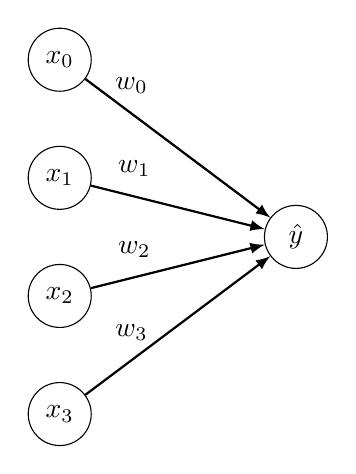
\begin{tikzpicture}[]

\begin{scope}[every node/.style={circle, draw, minimum size=8mm}]
    \node (x0) at (0, 0) {$x_0$};
    \node (x1) at (0,-1.5) {$x_1$};
    \node (x2) at (0,-3) {$x_2$};
    \node (x3) at (0,-4.5) {$x_3$};
    \node (y) at (3,-2.25) {$\hat{y}$};
\end{scope}

\begin{scope}[-latex, thick]
    \draw (x0) -- (y) node[pos=0.25, above, yshift=.8ex]{$w_{0}$};
    \draw (x1) -- (y) node[pos=0.25, above, yshift=.8ex]{$w_{1}$};
    \draw (x2) -- (y) node[pos=0.25, above, yshift=.8ex]{$w_{2}$};
    \draw (x3) -- (y) node[pos=0.25, above, yshift=.8ex]{$w_{3}$};
\end{scope}

\end{tikzpicture}
}
\end{document}
